\chapter{Overzicht van het thera project}
\label{hoofdstuk:overzicht}
Zoals eerder vermeld bouwt deze thesis verder op een reeds bestaand project. Om ze beter te kunnen situeren in het geheel is het handig om eerst even het thera project bekijken om zo te kunnen zien waar dit project in past.

\section{De opdelingen van het thera project}
Ruwweg gezien kan het reconstrueren van een fresco met behulp van de computer opgedeeld worden in 3~fasen.

\begin{description}
	\item[Acquisitie] Alle gevonden fragmenten worden ingescand met behulp van 3D en 2D-scanapparatuur om zo een virtueel model van elk stuk te bouwen, zie \cite{Brown2008}.  
	\item[Identificatie] Vervolgens worden deze virtuele fragmenten aan een zogenaamde \emph{matcher} gegeven, die voor elk fragmentenpaar gaat kijken of ze mogelijk op elkaar passen. Er zijn verschillende types ontwikkeld. E\'en ervan (genaamd \emph{RibbonMatcher} \cite{Brown2008}) kijkt enkel naar de randen van de brokstukken om te zien of ze in elkaar sluiten. Hierdoor is het in staat om passende fragmenten te vinden die voor mensen moeilijk te vinden zijn wegens te weinig distinctieve attributen zoals tekeningen. Het onderzoek gaat verder, in 2010 werd er een nieuw type ontwikkeld dat zijn analyse baseert op een combinatie van verschillende eigenschappen, zoals de sporen die een borstel kan nalaten bij het kleuren van een fresco of zelfs de beoordeling van de eerder genoemde \emph{RibbonMatcher} \cite{TolerFranklin2010}.
	\item[Classificatie \& Reconstructie] De derde en laatste stap bestaat uit het classificeren van wat de vorige stappen produceren. Elk voorgesteld paar moet gecontroleerd worden op validiteit. Verschillende statussen kunnen toegekend worden aan een paar, zoals: \emph{geconfirmeerd}, \emph{misschien}, \emph{nee}, \emph{in conflict met een ander paar}, et cetera. De \emph{matcher} produceert in de regel zeer veel mogelijk passende paren, waarvan slechts een klein deel correct kan zijn. De drempel voor het beslissen van wat een paar kan zijn en wat niet wordt in de vorige stap zo laag ingesteld omdat men wil vermijden dat twee fragmenten die toch passen genegeerd worden. Anders gezegd, de kost van ``\emph{false negatives}'' wordt hoog ingeschat. Uiteindelijk zal hieruit een gereconstrueerde fresco moeten ontstaan.
\end{description}

\section{Reconstructie, de bestaande oplossingen}
Het thesisproject besproken in deze tekst tracht de reeds bestaande hulpmiddelen van de reconstructiefase aan te vullen. Hievoor werden reeds programma's ontwikkeld, namelijk \emph{Griphos} en \emph{Browsematches}. Hierop volgt een bondige bespreking van beide programma's, wat ze kunnen en niet kunnen, en eventuele voor- en nadelen. Deze factoren hebben een belangrijke rol gespeelt bij het bepalen van de richting van deze thesis.

\subsection{Griphos}

Griphos was de eerste applicatie gericht op het weergeven en beoordelen van de resultaten van de voorgaande stappen. Het werd ontworpen met het doel een centraal zenuwstelsel te zijn voor alle informatie en met deze uiteindelijk een (zo goed mogelijk) gereconstrueerd fresco te maken. Het is mogelijk om zowel aparte fragmenten als automatisch herkende fragmentparen op een virtueel tafelblad te plaatsen en manipuleren (zie figuur \ref{fig:griphostafelblad}). De idee achter een dergelijke voorstelling komt voort uit een rechstreekse vertaling naar de computer van wat een archeoloog op een werkelijk tafelblad doet.\\

\begin{figure}[ht]
	\begin{center}
		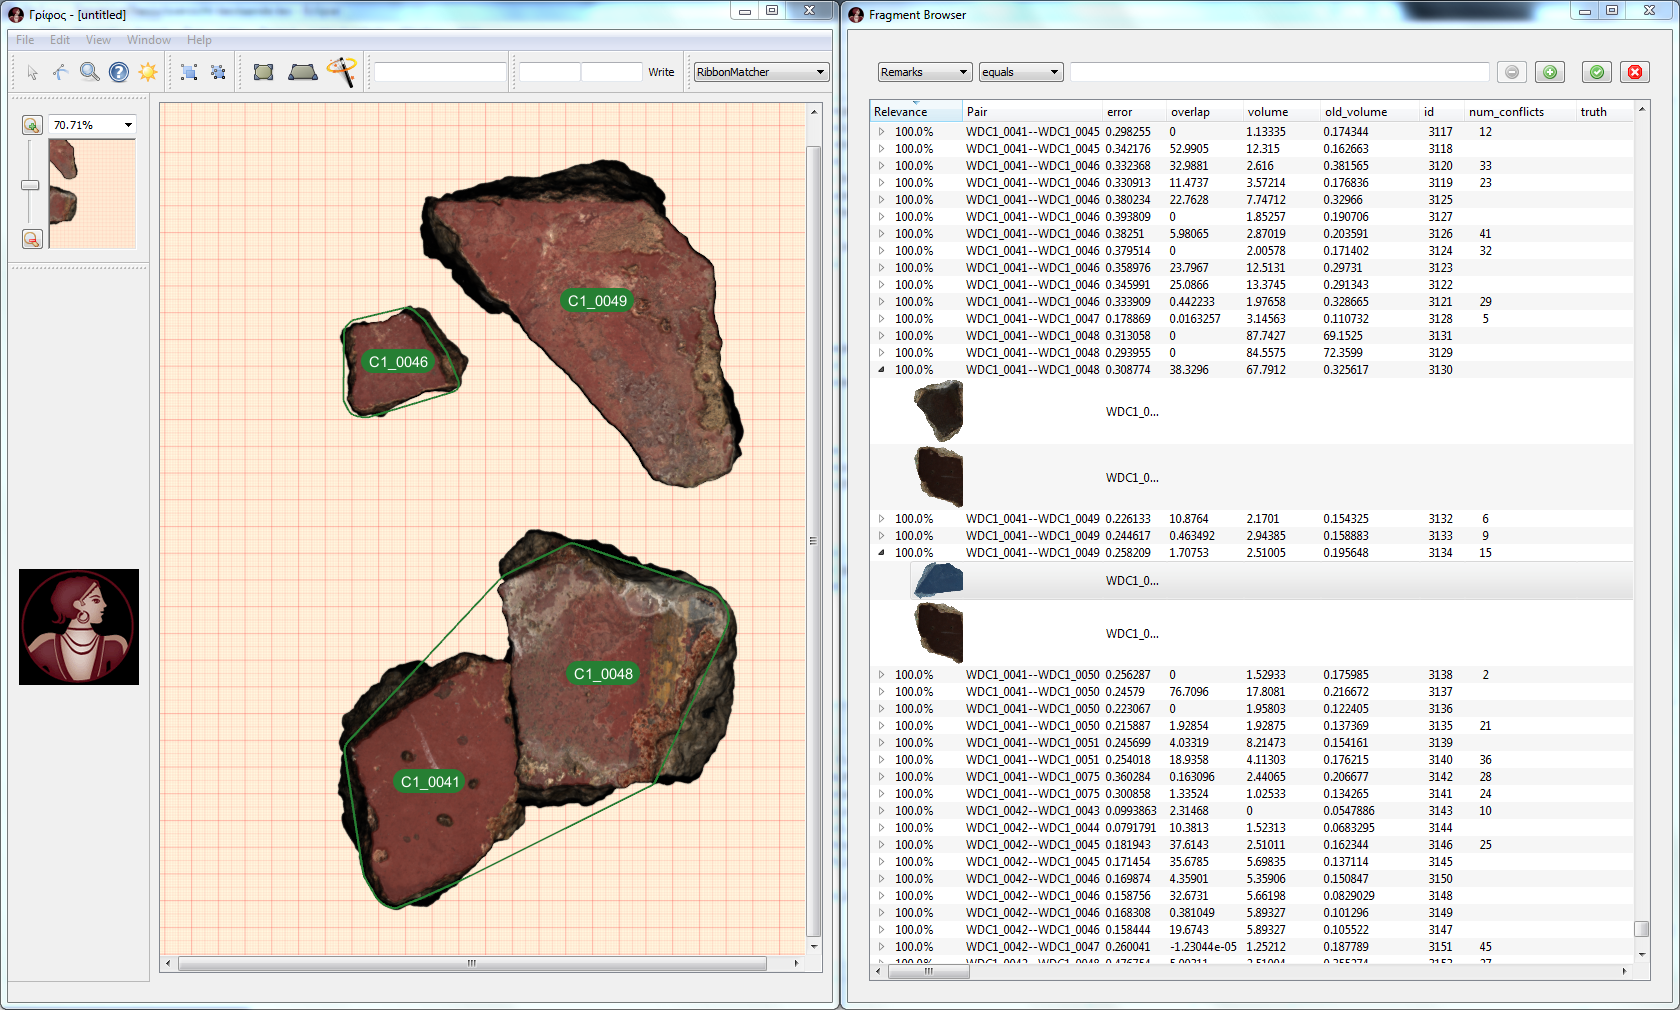
\includegraphics[width=.8\columnwidth]{images/griphos-01-cut.png}
		\caption{Een voorbeeld Griphos tafelblad, 1 voorgesteld paar en 2 aparte fragmenten zijn reeds ingeladen}
		\label{fig:griphostafelblad}
	\end{center}
\end{figure}

Griphos wordt echter geplaagd door een paar problemen: het is traag en biedt geen goede manier aan om de talloze gegenereerde paarvoorstellen na te kijken. De gebruikte metafoor van het virtuele tafelblad waarin gepuzzeld kan worden stelt een belangrijk deel van het reconstructieproces voor, maar schiet tekort als men de resultaten van automatische fragmentpaarontdekking op vloeiende wijze in het proces wil betrekken. Het probleem lijkt te zijn dat er te veel informatie is en Griphos geen goede manier aanbiedt om door de bomen het bos te zien. De aanzienlijke traagheid van sommige delen van het programma komen vooral voort uit de manier van dataopslag voor paren (XML bestanden) en de complexiteit van de visualisatie (afbeeldingen van hoge kwaliteit en/of gedetailleerde 3D-modellen). Dit zorgt voor een soms onaangename werkervaring zelfs indien men er toch in slaagt de juiste fragmentparen te lokaliseren. Desalniettemin is het een krachtig programma dat veel functionaliteit biedt voor de detailinspectie van brokstukken.\\

Het heeft zijn nut al op verschillende vlakken bewezen, behalve detailinspectie is het bijvoorbeeld ook in staat om de posities van fragmenten in een bak te onthouden. Dit betekent een grote snelheidswinst wanneer men bijvoorbeeld denkt een goed paar te hebben gevonden en men wil dit met echte fragmenten verifi\"eren. Als beide fragmenten in dezelfde bak liggen kan het correcte tafelblad ingeladen worden, Griphos kan vervolgens de gezochte fragmenten laten oplichten. Dit is veel effici\"enter dan fragmenten opsporen door vormen te vergelijken, zeker omdat de brokstukken vaak moeilijk te onderscheiden zijn zoals te zien valt in figuur \ref{fig:griphosbak}. 

\begin{figure}[ht]
	\begin{center}
		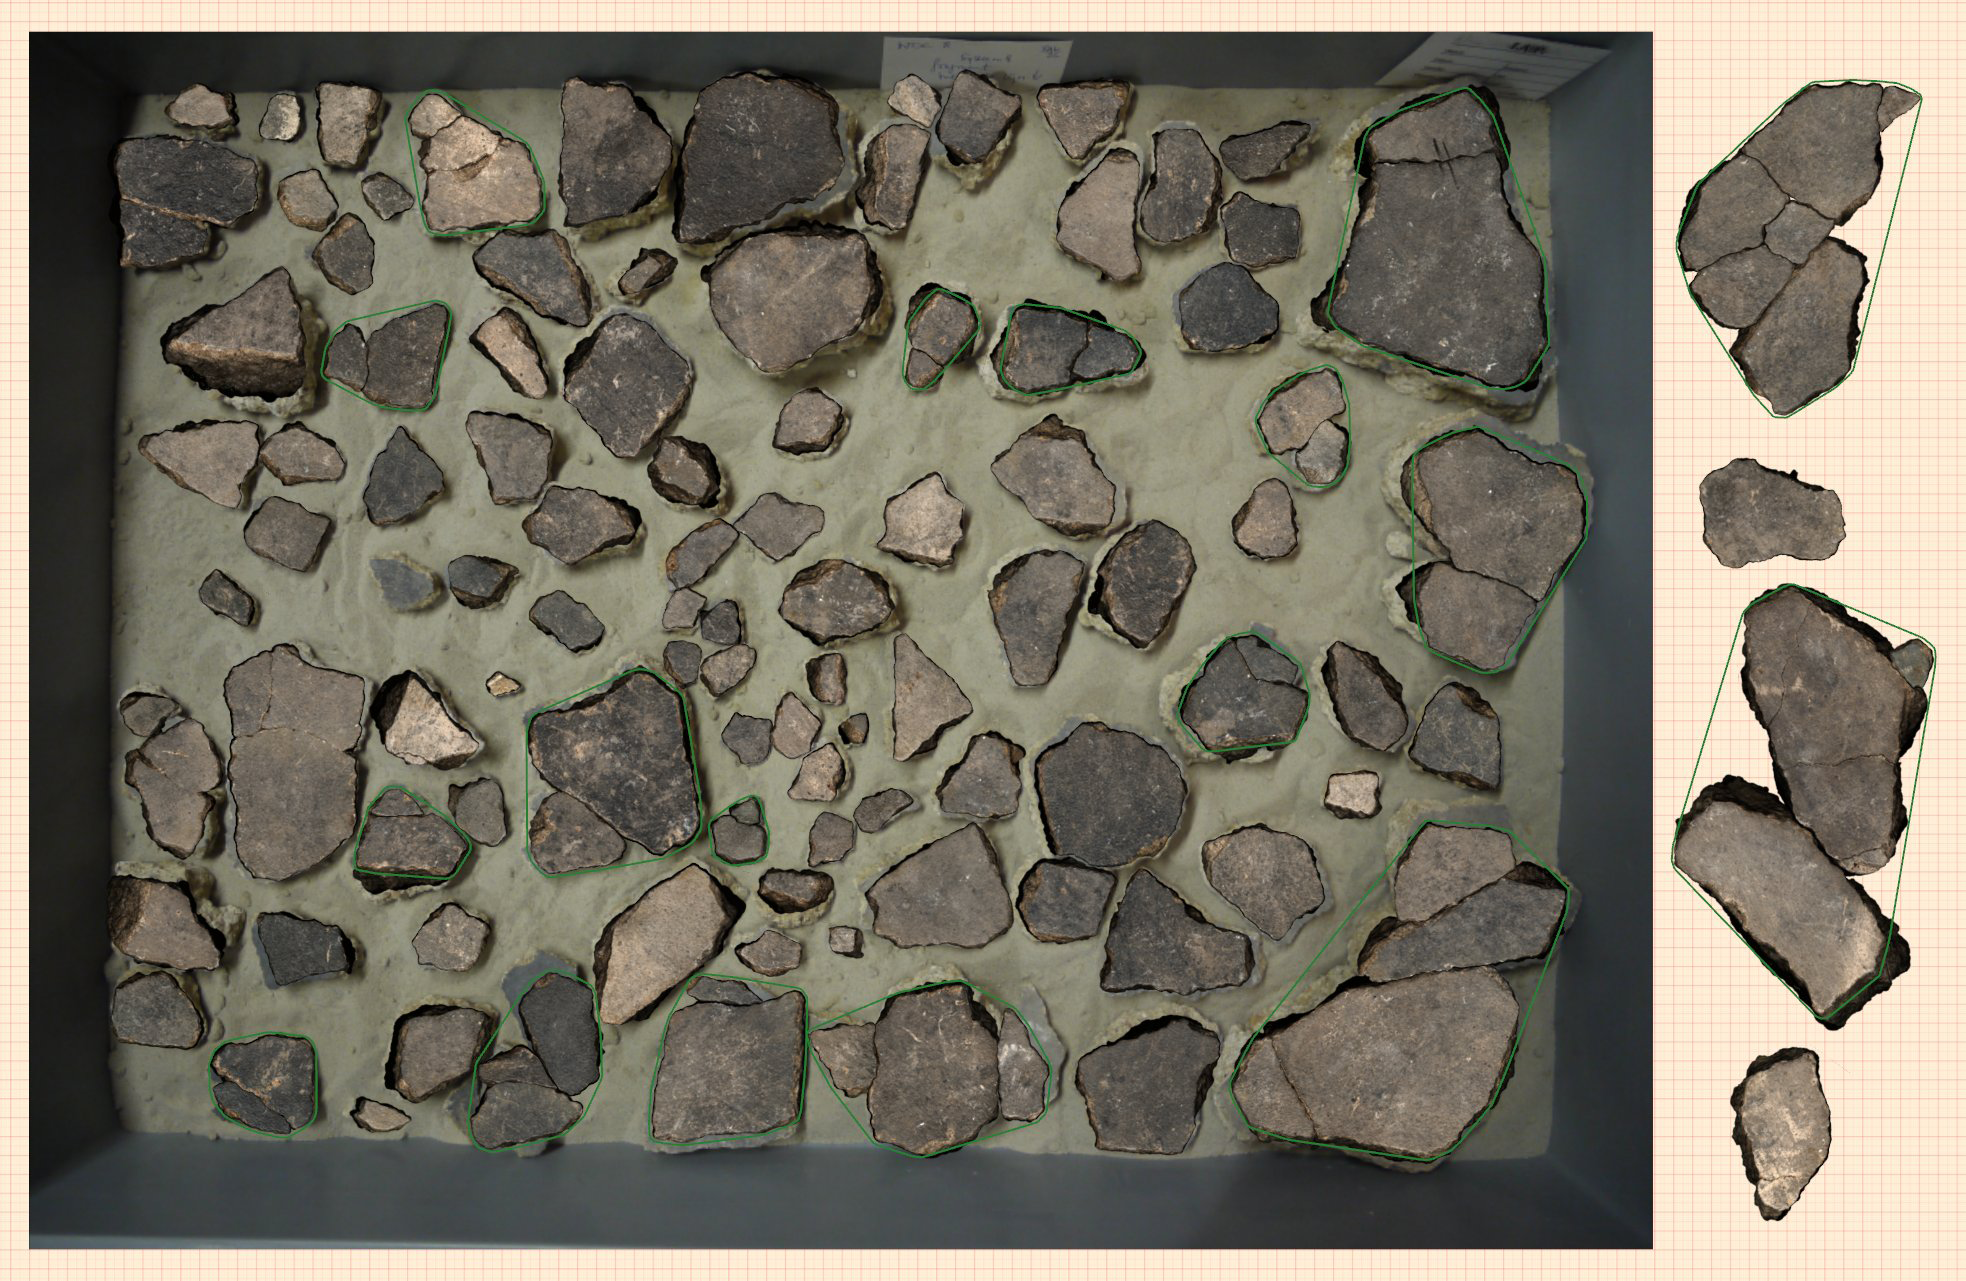
\includegraphics[width=.8\columnwidth]{images/griphos-bak-01.png}
		\caption{Griphos kan gebruikt worden om de posities van fragmenten in hun opslagplaats te onthouden en vervolgens snel terug te vinden. Het kan ook een foto van de bak waarin ze liggen onder het virtuele tafelblad projecteren. De brokstukken die buiten de bak staan weergegeven zijn verplaatst geweest naar een andere bak. (afbeelding met toestemming gebruikt uit \cite{Brown2011})}
		\label{fig:griphosbak}
	\end{center}
\end{figure}

// te technisch voor dit hoofdstuk, verplaats naar iets later: [TODO: remove]
Het eerste probleem wordt vooral veroorzaakt door trage datatoegang en te complexe visualisaties. Het programma slaagt alles betreffende paren op in een (enorm) XML bestand. Dit is nog doenbaar als men slechts een paar duizend voorstellen heeft maar ondervindt reeds snel onacceptabele vertragingen eens men er meer probeert in te laden. Ter voorbeeld, een kleine voorstellenverzameling van een bepaalde opgraving heeft er reeds 50000. Gekoppeld hieraan laadt Griphos ook steeds een hoge-kwaliteits afbeelding of zelfs een volledig 3D-model in voor elk paar De combinatie van het gebruik van grote XML-bestanden om informatie over de paren in op te slaan, en het steeds inladen van hoge kwaliteits-afbeeldingen en 3D-modellen. om alle info in op te slaan. Dit is bijzonder innefici\"ent en geeft ook bitter weinig mogelijkheden tot uitbreiding. Een ander deel is het gebrek aan zoekmogelijkheden binnen de voorstellen.

\subsection{Browsematches}

Een eerste prototype om de in Griphos ontbrekende delen aan te vullen, werd Browsematches genoemd. Het gebruikt eerst de visualisatiecapabilitieiten van Griphos om kleine afbeeldingen te nemen van elk bestaand paar met aan de linkerkant de doorsnede van hun raakvlak. Vervolgens toont het een scherm vol paren en kan men met de pijltoetsen navigeren tussen schermen. \\

\begin{figure}[ht]
	\begin{center}
		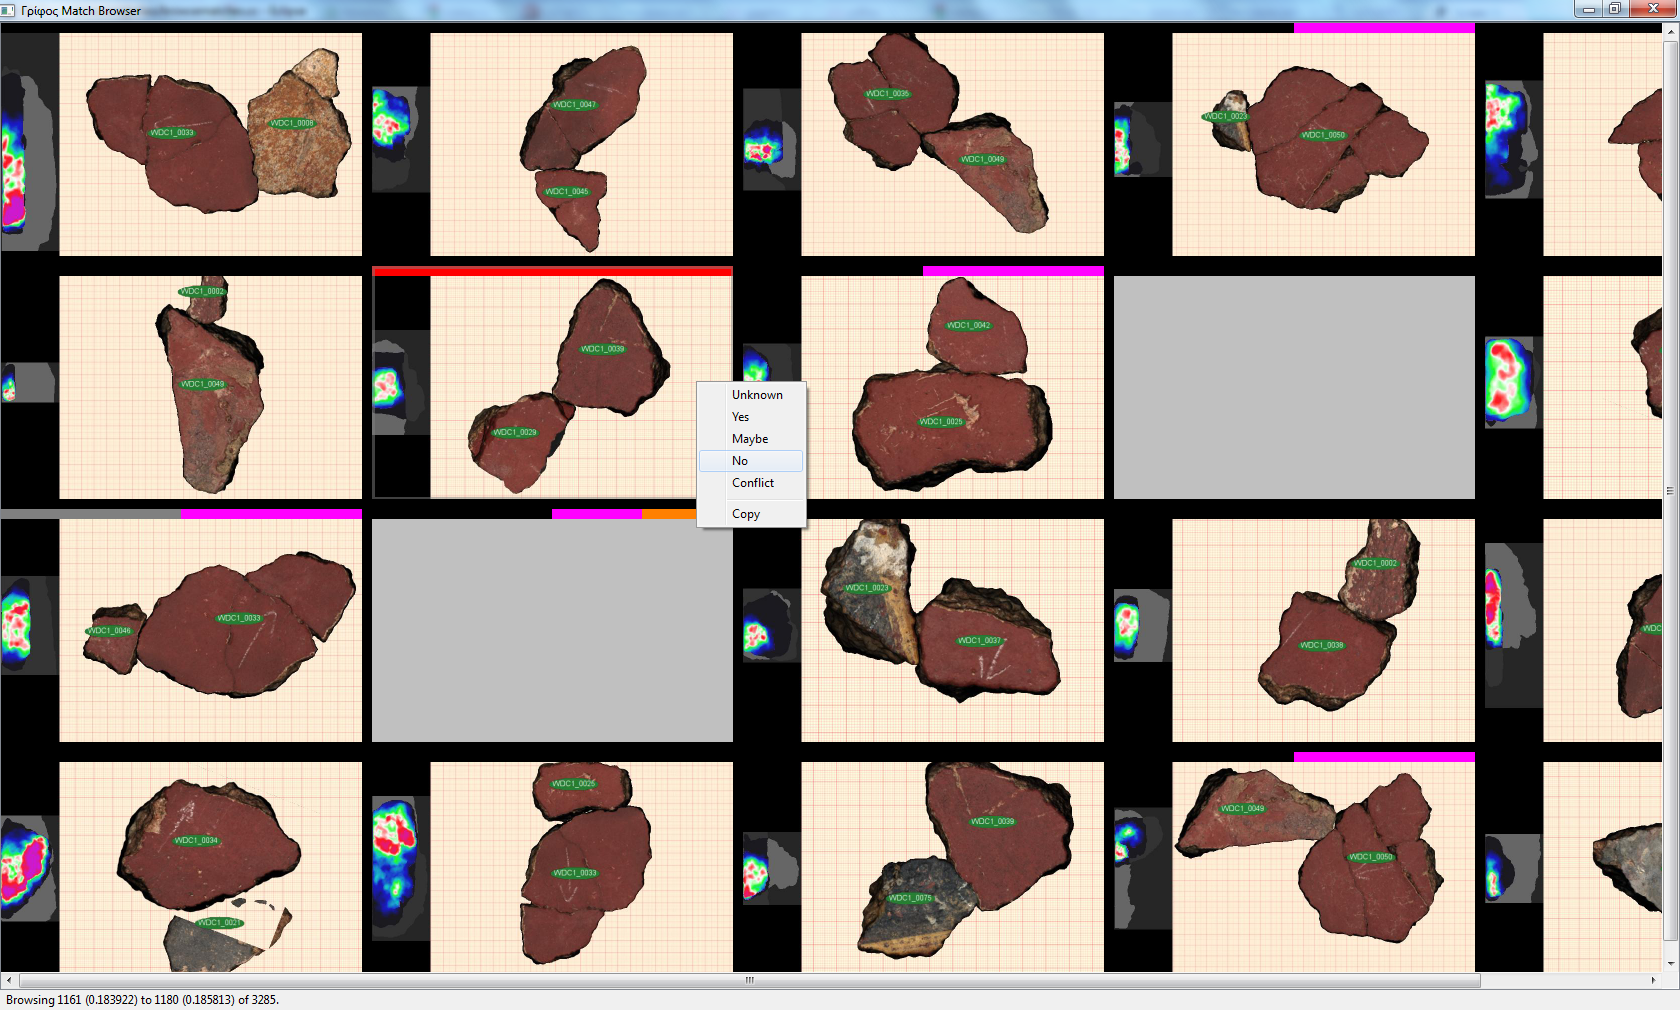
\includegraphics[width=.8\columnwidth]{images/browsematches-01-cut.png}
		\caption{Browsematches in werking, de balken boven de paren duiden een validatie door de gebruiker aan. Rood betekent bijvoorbeeld ``dit voorstel is zeker niet juist''}
	\end{center}
\end{figure}

Dit kleine programma groeide uit noodzaak: het valideren van paarvoorstellen is zo omslachtig met Griphos dat Browsematches in korte tijd in elkaar werd gestoken en succesvol werd gebruikt om het proces te stroomlijnen. Bij het begin van de thesis, om kennis te maken met het thera project, werd een verbinding gemaakt met Griphos zodat voorstellen die interessant waren in detail bestudeerd konden worden.\\

Browsematches erfde echter ook enkele van de nadelen van Griphos. Het inladen van de data is traag en vergt veel geheugen zelfs voor gereduceerde datasets. Daarbij is het moeilijk om de informatie uit te breiden of deze gemakkelijk te combineren met de bevindingen van andere onderzoekers. Daarenboven is Browsematches een prototype en niet bedoeld voor algemeen gebruik. Het simpele maar succesvolle concept diende als inspiratie en basis voor deze thesis. 

%%% Local Variables: 
%%% mode: latex
%%% TeX-master: "masterproef"
%%% End: 
